\chapter{Introduction}
\label{chap:introduction}

\chapterepigraph{The generation of fire by friction gave man for the first time control over one of the forces of nature, and thereby separated him for ever from the animal kingdom.}
{Friedrich Engels, \textit{Anti-Dühring} (1878)~\parencite{engels1878antiduhring}}

\glsresetall

This initial chapter provides a general introduction to this work.
It begins by presenting the research context that motivates the study.
It then introduces the research questions addressed throughout the thesis.
To address these questions, it then presents the main contributions.
Finally, it concludes with an overview of the structure of the thesis.

\section{Research Context}
\label{sec:introduction_research_context}

This section presents the context of this thesis.
We first introduce \gls{dl} and \gls{rl}, whose combination today enables highly capable agents.
We then discuss the alignment problem raised by such agents.
Next, we show how the \enquote{black-box} nature of \glspl{nn} makes this problem difficult to address.
Finally, we introduce \gls{me}, the approach adopted in this thesis to explain \gls{rl} agents.

\subsection{Deep Reinforcement Learning}

Over the past decade, \gls{ai} has advanced rapidly, driven largely by major developments in \gls{dl}.
This type of approach relies on artificial \glspl{nn}, which offer an unprecedented level of performance.
Inspired by their biological counterparts, these networks are known as connectionist models.
In such models, information is represented and transformed through patterns of interactions among interconnected elementary computational units \parencite{rumelhart1986learning}.

Among the fields transformed by \gls{dl}, \gls{rl} holds a particular place and is the main focus of this thesis.
The purpose of \gls{rl} is to enable an agent to learn how to make decisions through interactions with an environment \parencite{sutton2018reinforcement}.
At each step, the agent observes the current state of the environment and selects an action.
This action changes the state of the environment and results in a reward.
The objective of the agent is then to learn a behavior that maximizes the cumulative rewards obtained over time.

The combination of \gls{rl} and \gls{dl}, known as deep \gls{rl}, is currently the most effective approach for creating autonomous agents \parencite{arulkumaran2017deep}.
Due to their flexibility, \glspl{nn} provide a powerful means of representing the agent's information-processing capabilities.
Their use has consequently made it possible to apply \gls{rl} to problems that were previously intractable \parencite{mnih2013playingatarideepreinforcement, silver2017mastering, openai2019dota2largescale}.
The ability of \gls{rl} to operate in increasingly complex environments also allows agents to learn increasingly complex behaviors.
These behaviors are not explicitly programmed by the designer but emerge from the interaction between the learned policy, the environment, and the reward function.

\subsection{Alignment of Autonomous Agents}

As the capabilities of an agent increase, the resulting behaviors can become more difficult to anticipate and control.
In some cases, an agent may exploit unintended properties of its environment.

An illustrative example comes from agents trained to play hide-and-seek in a physics-based environment \parencite{baker2020emergent}, as shown in Figure~\ref{fig:hide_and_seek}.
In the intended course of the game, the blue hiders move boxes to block the entrances of their shelter.
They then lock these boxes in place so that the red seekers cannot get in, as shown in Figures~\ref{fig:hide_and_seek_boxes} and~\ref{fig:hide_and_seek_locked}.

However, the seekers also discovered an unintended strategy.
When the hiders barricade themselves in a corner, a seeker brings a ramp against the outer wall.
By running into the wall with this ramp at a specific angle, it launches itself into the air and lands behind the barricade, as shown in Figures~\ref{fig:hide_and_seek_ramp} and~\ref{fig:hide_and_seek_launch}.
This behavior, impossible under the intended rules of the environment, exploited a flaw in the physics engine that the designers had not anticipated.

\begin{figure}[t]
    \centering
    \begin{subfigure}[b]{0.48\textwidth}
        \centering
        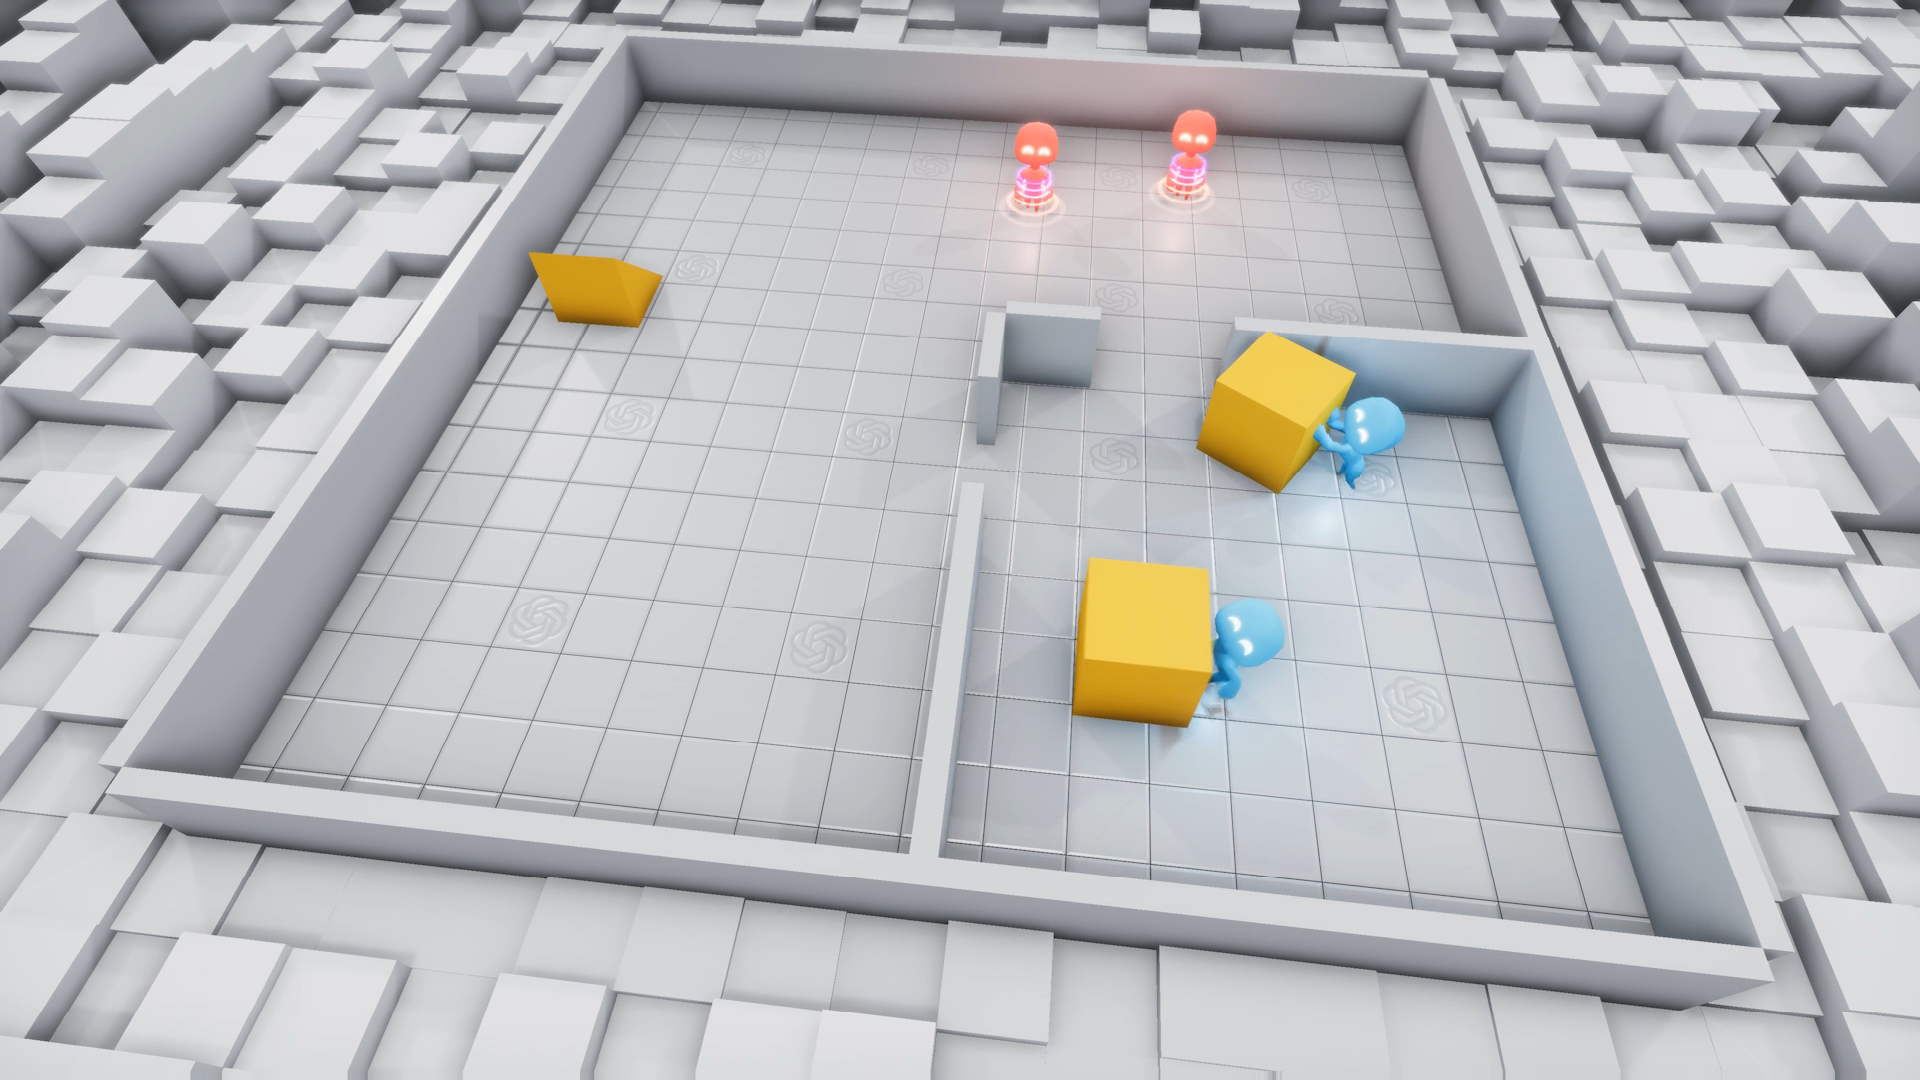
\includegraphics[width=\textwidth]{figures/introduction/hide_and_seek/hide_and_seek_boxes.png}
        \caption{}
        \label{fig:hide_and_seek_boxes}
    \end{subfigure}
    \hfill
    \begin{subfigure}[b]{0.48\textwidth}
        \centering
        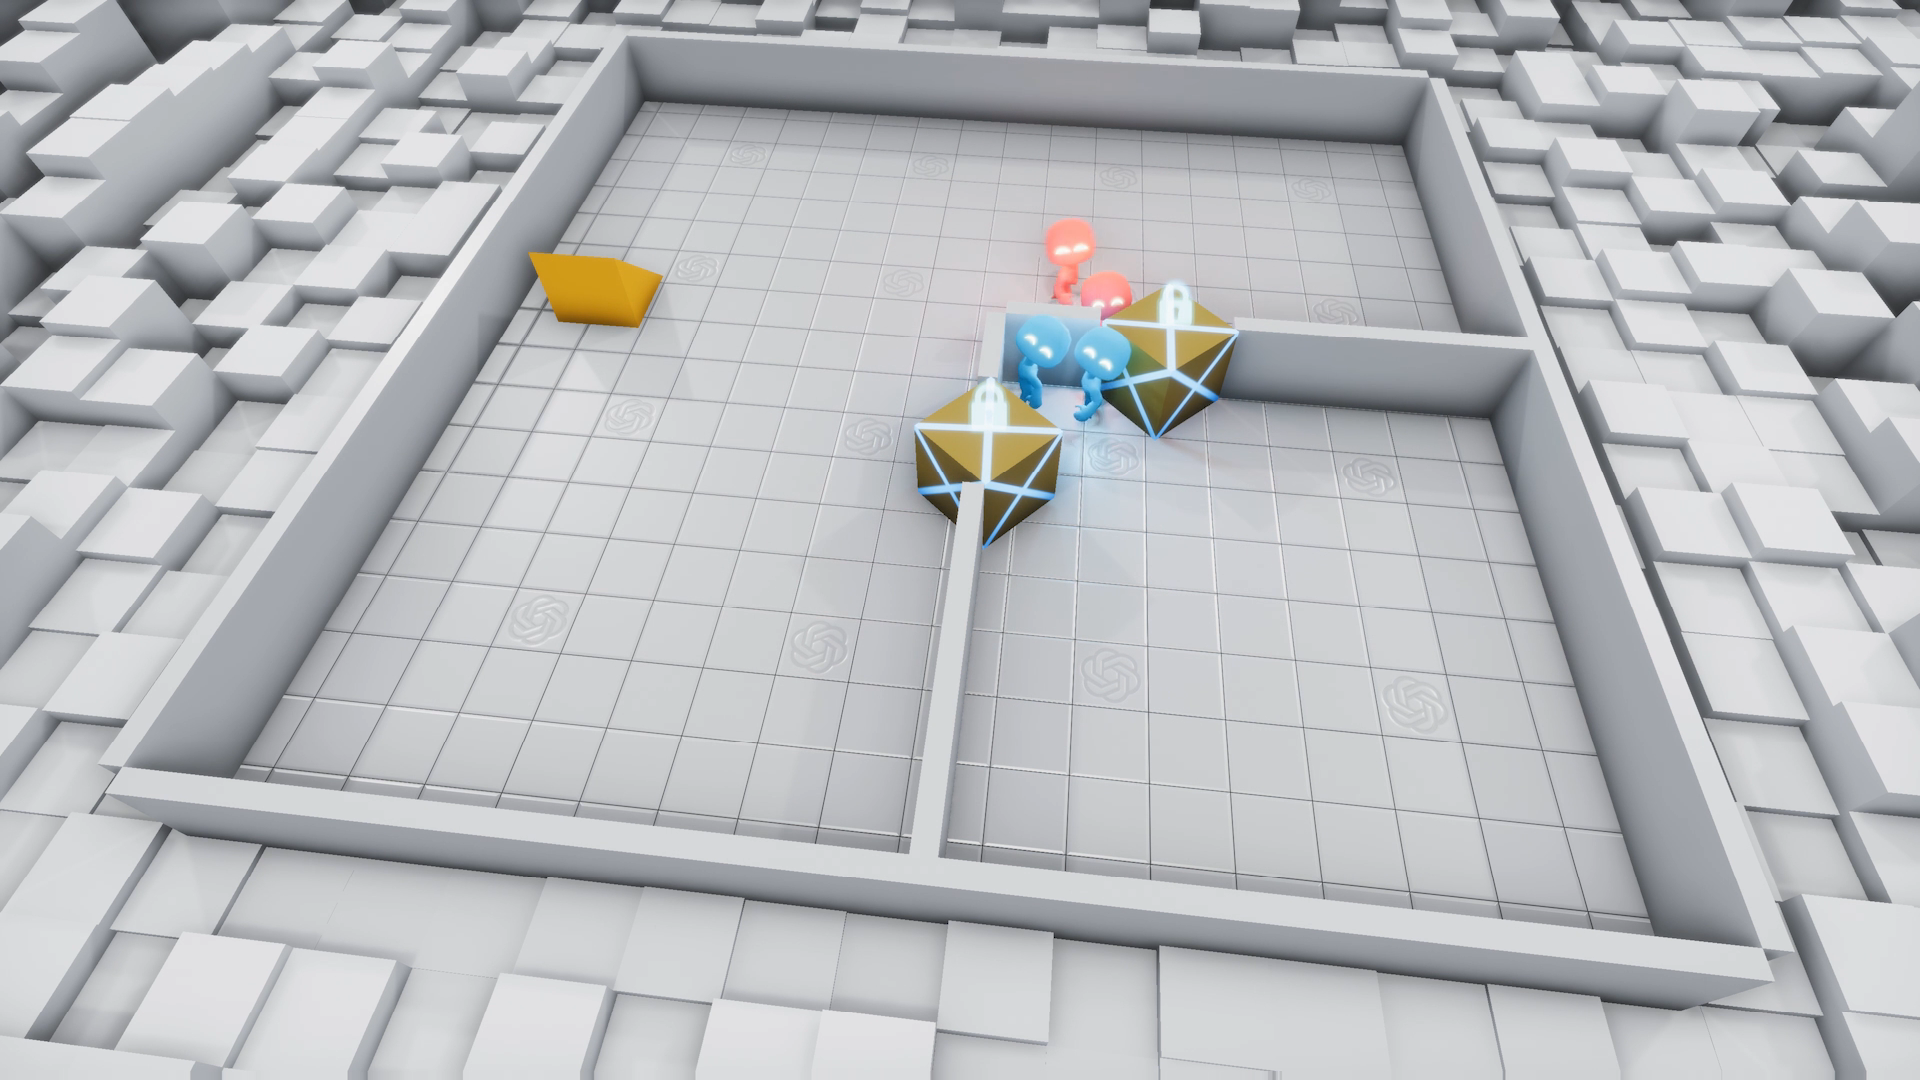
\includegraphics[width=\textwidth]{figures/introduction/hide_and_seek/hide_and_seek_locked.png}
        \caption{}
        \label{fig:hide_and_seek_locked}
    \end{subfigure}

    \vspace{0.5em}

    \begin{subfigure}[b]{0.48\textwidth}
        \centering
        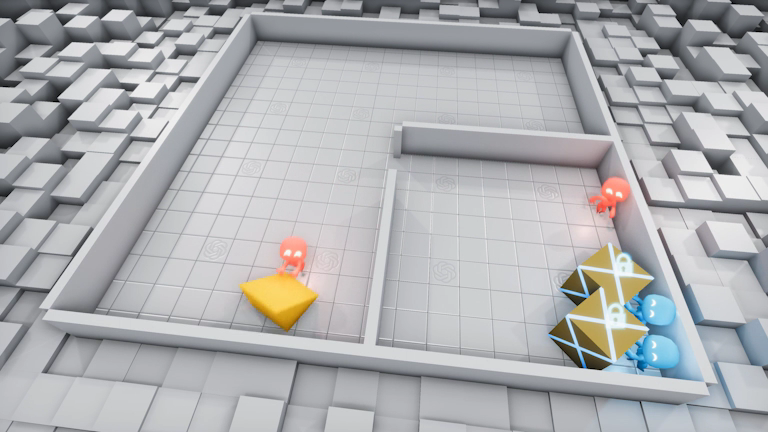
\includegraphics[width=\textwidth]{figures/introduction/hide_and_seek/hide_and_seek_ramp.png}
        \caption{}
        \label{fig:hide_and_seek_ramp}
    \end{subfigure}
    \hfill
    \begin{subfigure}[b]{0.48\textwidth}
        \centering
        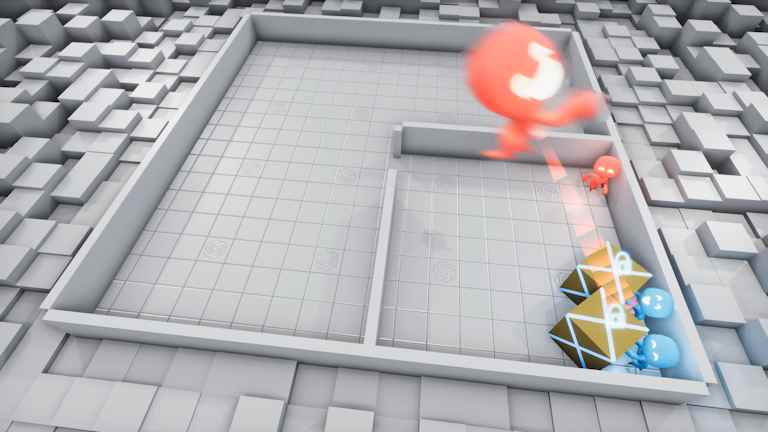
\includegraphics[width=\textwidth]{figures/introduction/hide_and_seek/hide_and_seek_launch.png}
        \caption{}
        \label{fig:hide_and_seek_launch}
    \end{subfigure}
    \caption[Agents playing hide-and-seek.]{Agents playing hide-and-seek \parencite{baker2020emergent}.}
    \label{fig:hide_and_seek}
\end{figure}


In a game environment, such behaviors have limited consequences.
However, agents trained with \gls{rl} are increasingly deployed in open-ended settings where they interact with the real world, notably \glspl{llm} trained with \gls{rl} and deployed as agents.
In such settings, a lack of control can have far more serious consequences.

Such behaviors relate to the problem of alignment (Definition~\ref{def:alignment}), which has become a central concern in \gls{ai} research \parencite{ji2023ai}.
The more capable agents become, the more pressing the need to ensure their alignment.

\begin{definition}{Alignment}{alignment}

Alignment is the problem of ensuring that the behavior of an \gls{ai} system corresponds to the intentions of its designers.

\end{definition}

\subsection{The Black-Box Problem}

The difficulty of ensuring the alignment of such agents stems in part from the fact that we only observe sequences of interactions between the agent and its environment.
These observations reveal how the agent's strategy is realized in particular situations.
However, understanding the strategy itself requires knowing how the agent would behave across all the situations it may encounter.
Since these situations are generally too numerous to be observed exhaustively, a collection of observed behaviors may not be sufficient to characterize the strategy.

To gain further insight into the agent's strategy, an alternative approach is to analyze the agent itself.
However, due to their connectionist nature, \glspl{nn} that model the agent's policy are not directly interpretable.
The information underlying a decision is distributed across many units and connections, making the processes leading to a decision difficult to trace.
\Glspl{nn} are therefore often regarded as \enquote{black-box} models \parencite{guidotti2018survey}.

\subsection{Mechanistic Explainability}

To address this \enquote{black-box} problem, the field of \gls{xai} has emerged \parencite{gunning2019darpa, arrieta2020explainable}.
In the specific context of \gls{rl}, this research area is referred to as \gls{xrl} \parencite{puiutta2020explainable, milani2022explainable}.
\gls{xrl} develops methods for producing explanations that improve our understanding of agent behavior.

These methods can be divided into two general approaches, which are detailed in Section~\ref{subsec:explainable_artificial_intelligence}.
Substitutive explainability adopts the \enquote{black-box} view and seeks to replace the \gls{nn} with alternative models that can be directly understood \parencite{rudin2019stop}.
Intrinsic explainability, in contrast, assumes that \glspl{nn} contain mechanisms that can be explained, the limitation being the lack of adequate tools to analyze them \parencite{olah2020zoom}.
This thesis adopts the intrinsic approach, and more specifically the one that seeks to explain the agent's strategy directly from the internal processes from which it emerges.
We refer to this approach as \gls{me} (Definition~\ref{def:mechanistic_explainability}).\footnote{Commonly referred to as \emph{mechanistic interpretability} \parencite{bereska2024mechanistic}. We use the term \emph{explainability} since the internal mechanisms of an \gls{nn} are not interpretable in the sense of Definition~\ref{def:interpretable}.}

\begin{definition}{Mechanistic Explainability}{mechanistic_explainability}

\gls{me} is the approach that seeks to explain an \gls{nn} by transforming its internal representations into interpretable information.

\end{definition}

\gls{me} is particularly promising because it addresses a core question of \gls{dl}, namely how an \gls{nn} processes information.
Explaining how an agent processes information to make its decisions would therefore improve not only our understanding of agent behavior, but also our understanding of \gls{dl} itself.
Such understanding is also a first step toward control \parencite{mini2023understanding}.

To understand how an \gls{nn} processes information, \gls{me} studies the intermediate representations it learns.
These representations are called \glspl{lr} \parencite{bengio2014representationlearningreviewnew}.
Together, they form the network's \gls{ls}.
Analyzing the structure of this \gls{ls} provides insights into how information relevant to decision-making is organized.
To develop an \gls{xrl} method based on \gls{me}, we need to address several research questions.
\section{Research Questions}
\label{sec:introduction_research_questions}

The first question concerns the analysis of \glspl{lr} themselves.
Numerous methods have been proposed to analyze the \glspl{ls}.
These methods originate from different research communities are rarely compared within a common framework.
This observation leads to our first research question:

\begin{researchquestion}{}{latent_space}
What approaches have been proposed in the literature to analyze the internal workings of \glspl{nn}?
\end{researchquestion}

The second question concerns the organization of existing research in \gls{xrl}.
Several taxonomies have been proposed to organize existing \gls{xrl} methods \parencite{puiutta2020explainable, milani2022explainable}.
However, these taxonomies often rely on approaches initially developed for explainability in supervised settings.
As a result, the organization of existing \gls{xrl} methods remains ambiguous, making it difficult to structure the field.
This observation leads to our second research question:

\begin{researchquestion}{}{taxonomy}
How can existing \gls{xrl} techniques be organized into a taxonomy that accounts for the specificities of \gls{rl}?
\end{researchquestion}

The analysis of existing \gls{xrl} approaches also reveals a third limitation.
Among existing methods for explaining \gls{rl} agents, few adopt a mechanistic perspective.
This observation leads to our third research question:

\begin{researchquestion}{}{mechanisms}
How can the internal representations of \glspl{nn} be exploited to identify the mechanisms underlying the decision-making process of \gls{rl} agents?
\end{researchquestion}

The analysis of existing \gls{xrl} methods highlights a fourth question concerning the evaluation of explanations.
There is no widely accepted set of objective criteria for evaluating the quality and relevance of the explanations produced by these methods.
Existing evaluations often rely on user studies or qualitative analyses, making it difficult to systematically assess the validity of an explanation approach \parencite{doshivelez2017rigorous, milani2022explainable}.
This leads to our fourth research question:

\begin{researchquestion}{}{evaluation}
How can the quality and relevance of explanations produced for \gls{rl} agents be objectively quantified?
\end{researchquestion}

\section{Contributions}
\label{sec:introduction_contributions}

To address these four research questions, this thesis is based on three main contributions.

The first contribution has not yet been published and addresses Research Question~\ref{rq:latent_space}.
In this contribution, we make explicit the working hypothesis that underlies much of the literature on \gls{ls} analysis.
We then organize existing \gls{ls} analysis methods into families to provide an overview of the different approaches.

The second contribution addresses Research Question~\ref{rq:taxonomy}.
This contribution takes the form of a first paper \parencite{alaarabiou:hal-04685607} and an extended English version \parencite{alaarabiou2026taxonomy}, both of which were submitted for review and accepted for publication.
In this contribution, we first clarify what explainability means in \gls{rl} by providing a clear frame of reference.
Building on these frame, we then conduct a comprehensive analysis of the state of the art in \gls{xrl}.

The third contribution addresses Research Questions~\ref{rq:mechanisms} and~\ref{rq:evaluation}.
In \textcite{alaarabiou2026car}, which has been reviewed and accepted for publication, we introduce \gls{car}, an \gls{xrl} method based on the principles of \gls{me}.
By analyzing the \glspl{lr}, \gls{car} produces explanations in the form of clusters of states that are similar from the agent's own perspective.
We further show that independently trained networks develop similarly structured representations, indicating that these representations reflect properties of the task rather than of a particular network.

This thesis can be viewed as a synthesis of these three contributions.

\section{Thesis Structure}
\label{sec:introduction_thesis_structure}

\begin{figure}[t]
    \centering
    \resizebox{\textwidth}{!}{
        \begin{tikzpicture}[
            chapter/.style={rectangle, draw, rounded corners, minimum height=1.6cm,
                            minimum width=2.9cm, align=center, font=\small, text width=2.7cm},
            legend/.style={rectangle, draw, rounded corners, font=\small,
                           inner xsep=8pt, inner ysep=5pt},
            >={Stealth},
            % Each category has its own color AND its own border style, so the
            % figure stays readable in grayscale: dashed for technical
            % background, solid for surveys, double line for the method.
            background/.style={draw=myblue,  fill=myblue!12, dashed, line width=1pt},
            survey/.style={draw=mygreen, fill=mygreen!12},
            method/.style={draw=myred,   fill=myred!12, double=myred!12,
                           double distance=1.6pt},
        ]

        % Chapter number (small, on top) followed by the chapter name in bold.
        \newcommand{\chapterbox}[2]{{\footnotesize Chapter~\ref{#1}}\\[3pt]\textbf{#2}}

        % Two parallel tracks, deep learning (top) and reinforcement learning
        % (bottom), which converge on the method chapter.
        \node[chapter, background]  (dl)   at (0, 1.1)   {\chapterbox{chap:deep_learning}{Deep\\Learning}};
        \node[chapter, survey] (ls)   at (3.5, 1.1) {\chapterbox{chap:latent_space_analysis}{Latent\\Space}};
        \node[chapter, background]  (rl)   at (0, -1.1)  {\chapterbox{chap:reinforcement_learning}{Reinforcement\\Learning}};
        \node[chapter, survey] (xrl)  at (3.5, -1.1){\chapterbox{chap:explainability_in_reinforcement_learning}{Explainability\\in \gls{rl}}};
        \node[chapter, method]   (car)  at (7.5, 0)   {\chapterbox{chap:clustering_agent_representations}{\gls{car}\\Method}};
        \node[chapter, method]   (exp)  at (11, 0)    {\chapterbox{chap:experiments}{Experiments}};

        % Within each track.
        \draw[->, thick] (dl)  -- (ls);
        \draw[->, thick] (rl)  -- (xrl);

        % Both tracks converge on the method chapter.
        \draw[->, thick] (ls.east)  -- ++(0.55, 0) |- ([yshift=0.35cm]car.west);
        \draw[->, thick] (xrl.east) -- ++(0.55, 0) |- ([yshift=-0.35cm]car.west);

        \draw[->, thick] (car) -- (exp);

        \matrix[ampersand replacement=\&, column sep=0.8cm, inner sep=0pt] at (5.5, -2.8) {
            \node[legend, background]  {Technical background}; \&
            \node[legend, survey] {Survey}; \&
            \node[legend, method]   {Method}; \\
        };

        \end{tikzpicture}
    }
    \caption{Structure of the thesis.}
    \label{fig:thesis_map}
\end{figure}


The thesis is organized into a sequence of chapters, with each chapter falling into one of these three categories:
\begin{itemize}
\item[] \textcolor{myblue}{\textbf{Technical background}} chapters introduce fundamental concepts required to understand the subsequent contributions.
\item[] \textcolor{mygreen}{\textbf{Survey}} chapters review the existing literature around a specific research question.
The organization adopted in each of these surveys is original and therefore constitutes a contribution of this thesis.
\item[] \textcolor{myred}{\textbf{Method}} chapters present \gls{car}, our \gls{me} method for \gls{rl}.
\end{itemize}

Following these categories, the chapters are organized as shown in Figure~\ref{fig:thesis_map} and detailed below:
\begin{description}[style=nextline, leftmargin=1.5em, itemsep=0.5em]
\item[\textcolor{myblue}{\textbf{Deep Learning (Chapter~\ref{chap:deep_learning}, technical background)}}]
This chapter introduces the fundamental concepts of \gls{dl}, the training paradigm used to optimize deep \glspl{nn}.
It begins with an overview of the historical developments that led to the emergence of the field.
It then formalizes the objective of \gls{dl} and describes the structure of artificial \glspl{nn}.
Next, it explains how the learning process shapes these networks and how the resulting models are evaluated.
It concludes by showing that \glspl{nn} progressively transform their inputs into intermediate representations, whose study motivates the following chapter.

\item[\textcolor{mygreen}{\textbf{Latent Space Analysis (Chapter~\ref{chap:latent_space_analysis}, survey)}}]
This chapter addresses Research Question~\ref{rq:latent_space} by providing a survey of existing approaches for analyzing the \glspl{ls}.
It first makes explicit the working hypothesis that underlies much of this literature, which we refer to as the \ConceptHypothesisName.
It then reviews four families of methods, based respectively on probing, interpretable directions, feature superposition, and clustering.
These families are compared within a common synthesis, which highlights their shared goal of understanding how information is organized in \glspl{lr}.
The chapter closes by discussing the absence of consensus on how to evaluate whether these methods truly capture the concepts of a model.

\item[\textcolor{myblue}{\textbf{Reinforcement Learning (Chapter~\ref{chap:reinforcement_learning}, technical background)}}]
This chapter introduces the fundamental concepts of \gls{rl}.
It begins with an overview of the milestones that led to the emergence of \gls{rl} as a unified field.
It then clarifies what is meant by an agent and formalizes the problem that \gls{rl} algorithms aim to solve.
Next, it explains how a policy is progressively refined through interaction with the environment to approach the optimal policy.
It concludes by showing how the combination of \gls{rl} and \gls{dl} gives rise to agents that are both powerful and difficult to understand.

\item[\textcolor{mygreen}{\textbf{Explainability in Reinforcement Learning (Chapter~\ref{chap:explainability_in_reinforcement_learning}, survey)}}]
This chapter addresses Research Question~\ref{rq:taxonomy} by reviewing existing approaches to explainability in \gls{rl}.
It first clarifies what is meant by an explanation in the context of \gls{xai}.
It then presents a taxonomy that categorizes \gls{xrl} methods according to the subject of the explanation, the source of information and the form it takes.
This taxonomy is used to structure a state-of-the-art.
The chapter concludes with three observations from this review: the absence of explanations of the learning process, a lack of unified evaluation metrics, and few intrinsic methods for explaining the deep neural policies.

\item[\textcolor{myred}{\textbf{The CAR Method (Chapter~\ref{chap:clustering_agent_representations}, method)}}]
This chapter addresses Research Questions~\ref{rq:mechanisms} and~\ref{rq:evaluation} by proposing \gls{car}, a new method for explainability in \gls{rl} based on the analysis of \glspl{lr}.
It first lays out the theoretical assumption underlying the method, which we term the \RepresentationConvergenceHypothesisName.
It then details the method itself, which extracts \glspl{lr} from surrogate policies and automatically detects \glspl{cs} through clustering.
Next, it introduces the \gls{cu}, \gls{as}, and \gls{acu} metrics, which evaluate the consistency and the abstraction of the resulting clusters without manual intervention.
Finally, it situates \gls{car} within the broader landscape of \gls{me}.

\item[\textcolor{myred}{\textbf{Evaluation of the CAR Method (Chapter~\ref{chap:experiments}, method)}}]
This chapter presents the implementation and experimental evaluation of the proposed method.
It first describes the software implementation of the \gls{car} pipeline and the experimental configuration, based on six environments from the Atari benchmark.
It then evaluates how faithfully the surrogate policies reproduce the behavior of the initial policy.
Next, a quantitative analysis measures the consistency and the abstraction of the clusters across the layers of the network.
Finally, a qualitative analysis examines the semantic content of the clusters, which capture aspects such as episode progression, specific game situations, and behavioral patterns.

\item[\textbf{Conclusion (Chapter~\ref{chap:conclusion})}]
This chapter closes the thesis by revisiting each research question in light of the contributions presented.
It then discusses the limitations of these contributions.
These limitations open several directions for future research, which are presented next.
Finally, the chapter ends with a broader reflection on this work.
\end{description}

The mathematical notation used throughout this thesis is summarized on page~\pageref{chap:notation}, and the acronyms are listed on page~\pageref{chap:acronyms}.

Finally, in the interest of transparency, we specify how generative \gls{ai} tools were used in this work.
\Glspl{llm} served as assistants during the preparation of this thesis.
They were used for writing tasks, including translation, wording improvement, and proofreading.
They were also used for software development, including code implementation and review.
Finally, they were used to support scientific work, including the identification of relevant documents and discussion of approaches.
They were not used as autonomous scientific sources.
All generated outputs were systematically reviewed, and the author takes full responsibility for the content presented in this thesis.

Now that the research context and objectives have been presented, we can turn to the first chapter, which introduces the fundamentals of \gls{dl}.
